%\documentclass{article}
\documentclass[12pt, oneside]{article}

\usepackage[letterpaper, scale=0.8, centering]{geometry}
\usepackage{fancyhdr}
\setlength{\parindent}{0em}
\setlength{\parskip}{1em}

\pagestyle{fancy}
\fancyhf{}
\renewcommand{\headrulewidth}{0pt}
\rfoot{{\footnotesize Copyright Mia Minnes, 2024, Version \today~(\thepage)}}

\usepackage{titlesec}

\author{CSE20S24}

\newcommand{\instructions}{{\bf For all HW assignments:} 
These homework assignments may be done individually or in groups of up to 3 students.
Please ensure your name(s) and PID(s)
are clearly visible on the first page of your homework
submission, start each question on a new page, and upload the PDF to Gradescope.
If you're working in a group, {\it submit only one submission per group}: one partner uploads the
submission through their Gradescope account and then adds the other group member(s) to the Gradescope submission
by selecting their name(s) in the ``Add Group Members'' dialog box. You will need to re-add your group member(s)
every time you resubmit a new version of your assignment.

Each homework question will be graded either for
{\bf correctness} (including clear and precise explanations and justifications of all answers) or
{\bf fair effort completeness}. You may collaborate on ``graded for correctness''
questions only with CSE 20 students in your group; if your
 group has questions about a problem, you may ask in drop-in help hours or post a private
post (visible only to the Instructors) on Piazza.  
 For ``graded for completeness''
 questions: collaboration is allowed with any CSE 20 students this quarter; 
 if your group has questions about a problem, you may ask in drop-in 
 help hours or post a public post on Piazza.

All submitted homework for this class must be typed. 
You can use a word processing editor if you like (Microsoft Word, Open Office, Notepad, Vim, Google Docs, etc.) 
but you might find it useful to take this opportunity to learn LaTeX. 
LaTeX is a markup language used widely in computer science and mathematics. 
The homework assignments are typed using LaTeX and you can use the source files 
as templates for typesetting your solutions.

{\bf Integrity reminders}
\begin{itemize}
\item Problems should be solved together, not divided up between the partners. The homework is
designed to give you practice with the main concepts and techniques of the course, 
while getting to know and learn from your classmates.
\item You may not collaborate on homework questions graded for correctness with anyone other than your group members.
You may ask questions about the homework in office hours (of the instructor, TAs, and/or tutors) and 
on Piazza (as private notes viewable only to the Instructors).  
You \emph{cannot} use any online resources about the course content other than the class material 
from this quarter -- this is primarily to ensure that we all use consistent notation and
definitions (aligned with the textbook) and also to protect the learning experience you will have when
the `aha' moments of solving the problem authentically happen.
\item Do not share written solutions or partial solutions for homework with 
other students in the class who are not in your group. Doing so would dilute their learning 
experience and detract from their success in the class.
\end{itemize}

}

\newcommand{\gradeCorrect}{({\it Graded for correctness}) }
\newcommand{\gradeCorrectFirst}{\gradeCorrect\footnote{This means your solution 
will be evaluated not only on the correctness of your answers, but on your ability
to present your ideas clearly and logically. You should explain how you 
arrived at your conclusions, using
mathematically sound reasoning. Whether you use formal proof techniques or 
write a more informal argument
for why something is true, your answers should always be well-supported. 
Your goal should be to convince the
reader that your results and methods are sound.} }
\newcommand{\gradeComplete}{({\it Graded for completeness}) }
\newcommand{\gradeCompleteFirst}{\gradeComplete\footnote{This means you will 
get full credit so long as your submission demonstrates honest effort to 
answer the question. You will not be penalized for incorrect answers. 
To demonstrate your honest effort in answering the question, we 
expect you to include your attempt to answer *each* part of the question. 
If you get stuck with your attempt, you can still demonstrate 
your effort by explaining where you got stuck and what 
you did to try to get unstuck.} }

%\usepackage{tikz}
%\usetikzlibrary{circuits.logic.US,circuits.logic.IEC}

\usepackage{amssymb,amsmath,pifont,amsfonts,comment,enumerate,enumitem}
\usepackage{currfile,xstring,hyperref,tabularx,graphicx,wasysym}
\usepackage[labelformat=empty]{caption}
\usepackage{xcolor}
\usepackage{multicol,multirow,array,listings,tabularx,lastpage,textcomp,booktabs}

% NOTE(joe): This environment is credit @pnpo (https://tex.stackexchange.com/a/218450)
\lstnewenvironment{algorithm}[1][] %defines the algorithm listing environment
{   
    \lstset{ %this is the stype
        mathescape=true,
        frame=tB,
        numbers=left, 
        numberstyle=\tiny,
        basicstyle=\rmfamily\scriptsize, 
        keywordstyle=\color{black}\bfseries,
        keywords={,procedure, div, for, to, input, output, return, datatype, function, in, if, else, foreach, while, begin, end, }
        numbers=left,
        xleftmargin=.04\textwidth,
        #1
    }
}
{}
\lstnewenvironment{java}[1][]
{   
    \lstset{
        language=java,
        mathescape=true,
        frame=tB,
        numbers=left, 
        numberstyle=\tiny,
        basicstyle=\ttfamily\scriptsize, 
        keywordstyle=\color{black}\bfseries,
        keywords={, int, double, for, return, if, else, while, }
        numbers=left,
        xleftmargin=.04\textwidth,
        #1
    }
}
{}

\newcommand\abs[1]{\lvert~#1~\rvert}
\newcommand{\st}{\mid}

\newcommand{\A}[0]{\texttt{A}}
\newcommand{\C}[0]{\texttt{C}}
\newcommand{\G}[0]{\texttt{G}}
\newcommand{\U}[0]{\texttt{U}}

\newcommand{\cmark}{\ding{51}}
\newcommand{\xmark}{\ding{55}}




%\usepackage{amsfonts,amssymb,amsmath,amsthm,color,comment,enumerate, graphicx,euscript,hyperref}
%\usepackage[makeroom]{cancel}
%\usepackage{paralist,listings}

\setlength{\evensidemargin}{0in}
\setlength{\oddsidemargin}{0in}
\setlength{\textwidth}{6.6in}
\setlength{\textheight}{8.8in}
\setlength{\topmargin}{0in}
\setlength{\footskip}{0.45in}
\renewcommand{\baselinestretch}{1}
\newlength{\saveparindent}
\setlength{\saveparindent}{\parindent}

% % NOTE(joe): This environment is credit @pnpo (https://tex.stackexchange.com/a/218450)
% \lstnewenvironment{algorithm}[1][] %defines the algorithm listing environment
% {   
%     \lstset{ %this is the stype
%         mathescape=true,
%         frame=tB,
%         numbers=left, 
%         numberstyle=\tiny,
%         basicstyle=\rmfamily\scriptsize, 
%         keywordstyle=\color{black}\bfseries,
%         keywords={,procedure, div, mod, for, to, input, output, return, datatype, function, in, if, else, foreach, while, begin, end, } %add the keywords you want, or load a language as Rubens explains in his comment above.
%         numbers=left,
%         xleftmargin=.04\textwidth,
%         #1 % this is to add specific settings to an usage of this environment (for instnce, the caption and referable label)
%     }
% }
% {}

% \newcommand{\A}[0]{\texttt{A}}
% \newcommand{\U}[0]{\texttt{U}}
% \newcommand{\G}[0]{\texttt{G}}
% \newcommand{\C}[0]{\texttt{C}}

\newif \ifsolution
\solutiontrue
\solutionfalse

\newcommand{\sol}[1]{\medskip\fbox{\begin{minipage}{5.5in}{#1}\end{minipage}}\medskip}

\begin{document}
\begin{center}
{\Large
CSE 20 Spring 2024\\ 
Practice for Test 1 \ifsolution{\qquad Solutions}\fi}
\end{center}

\thispagestyle{empty}

\ifsolution{}
\else{}
Below are the instructions that will be on the first page of the test package:

\begin{center}
  \begin{minipage}[t]{7in}
  \rule{\linewidth}{2pt}
  \textbf{INSTRUCTIONS --- READ THIS NOW}
  \begin{itemize}
  
  \setlength{\itemsep}{0.025in}
  
  \item  Write your name, PID, current seat number, exam time, 
  and the academic integrity pledge in the indicated space above and 
  on the designated  {\bf answer sheet}.
  We will check for {\bf all} of this identifying information before grading.
  Write your answers in the specified areas, or your work will not be graded. 
  
  \item We will not be answering questions about the exam during the exam period. 
  If any bugs are found in the exam after the exam period, the affected question part(s) will be addressed.
  
  \item  You may use one 8.5"x11", doublesided sheet of notes that you create and bring to the exam room, but no other books, notes, or aids.
  
  \item You may not speak to any other student in the exam room while the exam 
  is in progress (including after you hand in your own exam).  You may not share
  {\bf any information} about the exam with anyone who has not taken it.
  
  \item Turn off and put away all cellphones, calculators, and other electronic devices.
  You may not access any electronic device during the exam period. If you need to leave 
  the room during the exam period, you must leave all electronic devices with an exam proctor.
  
  \item  To receive full credit, your answers must
  be written neatly, legibly, and sufficiently darkly to scan well in the indicated answer box. Your solution will be evaluated both for correctness and clarity.
  Read the instructions for each part carefully to determine what is required for full credit.
  This test has $??$ problems worth a total of $??$ points.
  
  \item This exam is {\bf 45 minutes} long. Read all the problems first before you start 
  working on any of them, so you can manage your time wisely.
  
  \item Please stay seated until the end of the exam period.
  We will collect all exams and note sheets at the {\bf end} of the exam period, to minimize disruption 
  for students who wish to use the full time for the exam. Please show your ID to a proctor when you hand 
  in your exam. 
  
  
  \end{itemize}
  \end{minipage} \hfill
  \end{center}
  \newpage
\fi

\begin{description}

\item[1. Modeling, Sets and Functions, Algorithms] 
In machine learning, clustering can be used to group similar data for prediction and recommendation.  For example,
each Netflix user's viewing history can be represented as a $n$-tuple indicating their preferences about
movies in the database, where $n$ is the number of movies in the database.  Each element in the $n$-tuple indicate
the user's rating of the corresponding movie: 
$1$ indicates the person liked the movie, $-1$
that they didn't, and $0$ that they didn't rate it one way or another.

Consider the following algorithm for determining if a user's viewing history represents
strong opinions on many movies.
\begin{algorithm}[caption={Determine if user's ratings tuple encode strong opinions}]
procedure $\textit{opinion}$($(r_1, \ldots, r_n)$: a $n$-tuple of ratings; $c$: a nonnegative integer)
$sum$ := $0$
for $i$ := $1$ to $n$
  if $r_i \neq 0$
    $sum$ := $sum + 1$
return $sum \geq c$
\end{algorithm}

  \begin{enumerate}%[(a)]
  \item When $n = 3$, describe the set of all $n$-tuples representing user ratings
  \begin{enumerate}%[i.]
  \item By the roster method.
  
  \ifsolution{
  \sol{There are 27 $3$-tuples whose elements are each $-1$, $0$, or $1$.  We can list them as follows.
  \begin{align*}
  \{ & (-1, -1, -1) , (-1, -1, 0) , (-1, -1, 1) , (-1, 0, -1), (-1, 0, 0), (-1, 0, 1),\\
     & (-1, 1, -1), (-1, 1, 0), (-1, 1, 1), (0, -1, -1) , (0, -1, 0) , (0, -1, 1) , \\
     & (0, 0, -1), (0, 0, 0), (0, 0, 1), (0, 1, -1), (0, 1, 0), (0, 1, 1), (1, -1, -1) , \\
     & (1, -1, 0) , (1, -1, 1) , (1, 0, -1), (1, 0, 0), (1, 0, 1), (1, 1, -1), (1, 1, 0), (1, 1, 1) \}  
  \end{align*}
  }}\fi
  
  \item With set builder notation.
  
  \ifsolution{
  \sol{Using set builder notation, we can specify the constraints on each component of the $3$-tuple:
\[
	\{ (x,y,z) ~\mid~ x \in \{-1,0,1\}~\text{and}~ y\in \{-1,0,1\}~\text{and}~ z \in \{-1,0,1\} \}
\]  
}}\fi
  
  \item Using a recursive definition.
  
  \ifsolution{
  \sol{  Let's call the set of ratings of three movies $R_3$. We can define this set recursively 
  by listing each of the finitely many tuples in $R_3$ in the basis step and then 
  defining the recursive step to be: when $u \in R_3$, so is $u$.

  Note that this recursive definition is somewhat contrived: the recursive step isn't doing anything helpful.
  }}\fi
  \end{enumerate}
 \item What are the possible return (output) values of this algorithm?
  
  \ifsolution{
  \sol{ Since the algorithm returns the result of a comparison, the possible values are 
  True or False.}
  }\fi
  
  \item {\bf Trace} the computation of $opinion( (-1, 0, 0, 0, 1, 1,-1), 2)$.

\ifsolution{\sol{
The computation of $opinion( (-1, 0, 0, 0, 1, 1,-1), 2)$  first (in line 2) initializes
the variable $sum$ to $0$ and then steps through each component of the tuple in the for 
loop in line 3, checking (in line 4) if the value is zero or not. The first component
of $(-1, 0, 0, 0, 1, 1,-1)$ is nonzero so line 5 increments $sum$, which now has value $1$.
When the for loop checks the components at positions 2,3,4, the $sum$ variable is not updated.
When the for loop 
gets to each of positions 5,6,7, the nonzero value of the elements at these positions means the 
if branch of the condition is followed and the $sum$ variable is incremented three times, to 
get to the value $4$.  In line $6$, the comparison $sum \geq c$ evaluates to $4 \geq 2$, which is True.
Thus, $opinion( (-1, 0, 0, 0, 1, 1,-1), 2)$ returns True.
}}\fi

  \item Give an example of a nonnegative integer $c$ so that, no matter which $n$-tuple
  $(r_1, \ldots, r_n)$ we consider, $opinion( (r_1, \ldots, r_n), c)$ will have the same value.
  What value is it?

\ifsolution{\sol{The nonnegative integer $c = 0$ is an example.  The value of $sum$ is initialized to $0$ in line 2. 
The values of the components $n$-tuple $(r_1, \ldots, r_n)$ determine whether the value of $sum$ ever increases in the form loop lines 3-5; the value can never decrease. Thus, no matter the choice of $n$-tuple,
 the comparison $sum \geq 0$ will evaluate to True.
}}\fi


\end{enumerate}

\item[2. Sets and Functions] \qquad \\
\begin{enumerate}%[(a)]
\item Give a recursive definition for the set $\mathbb{N}$.

\ifsolution{\sol{The set of nonnegative integers can be defined recursively as follows:

Basis step: $0 \in \mathbb{N}$

Recursive step: If $x \in \mathbb{N}$ then $x+1 \in \mathbb{N}$.
}}\fi

\item Use the recursive definition from part (a) to give a recursive definition for the function with domain $\mathbb{N}$, codomain
$\mathbb{N}$ which computes, for input $i$, the sum of the first $i$ powers of $2$.  For example, on input $0$, the function 
evaluates to $2^0$, namely to $1$.  On input $1$, the function evaluates to $2^0 + 2^1$, namely $3$. 
On input $2$, the function evaluates to $2^0 + 2^1 + 2^2$, namely $7$. 

\ifsolution{\sol{Let's call this function $sumPow$.  Its recursive definition will mirror the recursive definition of its domain, from part (a).

$sumPow: \mathbb{N} \to \mathbb{N}$

Basis step: $sumPow(0) = 1$.

Recursive step: If $x \in \mathbb{N}$ then $sumPow(x+1) = sumPow(x) + 2^{x+1}$.

In this function definition, we assumed that we have access to a definition of the power function
to compute powers of two. In fact, we can define this
function recursively as well:

$powTwo: \mathbb{N} \to \mathbb{N}$

Basis step: $powTwo(0) = 1$.

Recursive step: If $x \in \mathbb{N}$ then $powTwo(x+1) = 2 powTwo(x) = powTwo(x) + powTwo(x)$.

}}\fi
\end{enumerate}

\item[3. Base expansions, Multiple representations] \qquad \\
\begin{enumerate}%[(a)]
\item Compute the ternary (base 3) expansion of $28$.

\ifsolution
\sol{
We can express $28$ in terms of powers of $3$ as 
\[
28 = 1 \cdot 27 + 1  = 1 \cdot 3^3 + 0 \cdot 3^2 + 0 \cdot 3^1 + 1 \cdot 3^0 = (1001)_3.
\]
Therefore, by definition of base $3$ expansion, $28 = (1001)_3$.
}
\else{}
\fi
\item Compute the product of $(6A)_{16}$ and $(11)_{16}$, without converting
either number to another base.

\ifsolution
\sol{
We use the usual algorithm for multiplication, except using hexadecimal symbols.

\begin{align*}
   &6A \\
\underline{\times~ }&\underline{11} \\
& 6A \\
\underline{+6~}&\underline{A0} \\
7&0A
\end{align*}

Thus, the product of $(6A)_{16}$ and $(11)_{16}$ is $(70A)_{16}$.
}
\else{}
\fi

\item Confirm your answer for part (b) by converting $(6A)_{16}$ and $(11)_{16}$ to
decimal, multiplying them, and converting the product to base $16$.

\ifsolution
\sol{
Converting:
\[
(6A)_{16} = 6  \cdot  16^1 +  10 \cdot 16^0  = 96 +  10 =  106
\]
\[
(11)_{16} = 1 \cdot 16^1 +  1 \cdot 16^0  = 16+  1 =  17
\]
Multiplying in decimal:

\begin{align*}
   &106 \\
\underline{\times~ }&\underline{~17} \\
& 742 \\
\underline{+1}&\underline{060} \\
1&802
\end{align*}

Converting back to hexadecimal:  by long  division, 
\begin{align*}
1802 &= 112\cdot 16  + 10 \\
112  &= 7 \cdot 16 +  0\\
7 &= 0 \cdot 16 + 7
\end{align*}
Thus, $1802  = (70A)_{16}$, agreeing  with part (b).
}

\else{}
\fi

\item How many bits will there be in the binary (base $2$) expansion of $2020$?  Can you compute this
without fully converting $2020$ to base $2$?


\ifsolution
\sol{
The  leading coefficient will need to be in the column  corresponding to the highest power  of $2$ less
than  or equal to   $2020$. Listing the powers of $2$:
\begin{center}
\begin{tabular}{|l|c|c|c|c|c|c|c|c|c|c|c|c|c|}
\hline
Exponent & $0$ & $1$ & $2$ &  $3$  &  $4$  & $5$ & $6$ & $7$ & $8$ & $9$ &  $10$ & $11$\\
\hline
Power &$1$ & $2$ & $4$ &  $8$  &  $16$  & $32$ & $64$ & $128$ & $256$ & $512$ &  $1024$ & $2048$\\
\hline
\end{tabular}
\end{center}
we see  that the binary expansion of $2020$  will  be of the  form  $(1a_{9} \cdots a_0)_{2}$ and will therefore
have $11$ bits.
}
\else{}
\fi

\item Give an example of a number that can be represented in base 2 fixed-width 3,
but not in base 2 expansion.

\ifsolution
\sol{
The number  $0$ can't be  represented in binary (base 2)  but is represented in base $2$ fixed-width $3$
$(000)_{2,3}$.
}
\else{}
\fi

\item Give an example of a number that can be represented in
base 2 expansion, but not in base 2, fixed-width 3 expansion.

\ifsolution
\sol{
The number $8$ can be  represented in base  $2$ as $(1000)_2$ but can't be represented in 
binary fixed-width $3$ because it requires four bits.}
\else{}
\fi

\item Give the representation of -7 in sign-magnitude width 3 and 2s complement
width 3. Then do the same for width 4.

\ifsolution
\sol{
The  number $-7$ can't be represented in sign magnitude width 3 or in 2s complement width 3:
\begin{itemize}
\item The least number that can be represented in sign magnitude width 3 has representation $[111]_{s,3}$ 
and is  $-3$.
\item The least number that can be represented in 2s complement width 3 has representation $[100]_{2c,3}$ 
and is  $-4$.
\end{itemize}
With width 4 we can use the following representations:
\begin{itemize}
\item In sign magnitude width 4, $-7$ has representation $[1111]_{s,4}$  because the leftmost bit  is the 
sign bit and the magnitude  of $-7$ has binary fixed width 3 representation $7 = (111)_{2,3}$.
\item In 2s complement width 4, $-7$ has representation $[1001]_{2c,4}$  because the leftmost bit  is the 
sign bit and rightmost bits need to  represent $2^{4-1}-7 = 1$ in binary fixed width 3, $(001)_{2,3}$.
Alternatively, we calculate that $[1001]_{2c,4} = 1 \cdot (-2)^3 + 0 \cdot 2^2 + 0 \cdot 2^1 + 1 \cdot 2^0 = -8 + 1 = -7$.
\end{itemize}
}
\else{}
\fi

\item Give the representation of 10.5625 in fixed-width base-2 expansion with
integer width 4 and fractional width 9.

\ifsolution
\sol{
We need  to write $10.5625$ as 
\[
(a_3 a_2 a_1 a_0.c_1  c_2 c_3  c_4 c_5  c_6 c_7 c_8 c_9)_{2,4,9}
\]
For the integer part:  $10 = 1\cdot 2^3 +  0 \cdot 2^2 + 1 \cdot 2^1 + 0 \cdot  2^0 = (1010)_2$

For the fractional part: $0.5625 =  1\cdot 2^{-1}  +  0 \cdot  2^{-2} + 0 \cdot 2^{-3} + 1 \cdot 2^{-4} $
where
\begin{center}
\begin{tabular}{|l|c|c|c|c|c|c|c|c|}
\hline
Exponent & $-1$ & $-2$ & $-3$ &  $-4$  &  $-5$ & $-6$ & $-7$ \\
\hline
Power &$0.5$ & $0.25$ & $0.125$ &  $0.0625$  &  $0.03125$  & $0.015625$ & $0.0078125$\\
\hline
\end{tabular}
\end{center}
Thus, 
\[
10.5625 = (1010.100100000)_{2,4,9}
\]
}
\else{}
\fi
\end{enumerate}


\item[4. Circuits]   
A triangular number (or triangle number) counts the objects that can form an equilateral
triangle, as in the diagram below. The $n^{\text{th}}$ triangular number is the sum of the first $n$
 integers,
as shown in the following figure illustrating the first four triangular numbers (what is the
fifth one?):
\begin{center}
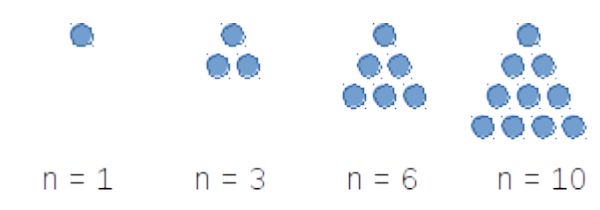
\includegraphics[width=2.7in]{../../resources/images/triangle.png}
\end{center}
Design a circuit that takes four inputs $x_0, x_1, x_2, x_3$ and outputs
True (T or 1) if the integer value 
$(x_3x_2x_1x_0)_{2,4} $ is a triangular number, and False (F or 0) otherwise. You may assume that 0 is
not a triangular number. ({\it Credit: UBC Department of Computer Science})

\ifsolution{
\sol{
Using the definition, we can write a table of values for the circuit we need to build, since the output will be 
one when $(x_3 x_2 x_1 x_0)_{2,4}$ will be one of $1, 3, 6, 10, 15$.
\begin{center}
\begin{tabular}{cccc||c}
$x_3$& $x_2$ & $x_1$ & $x_0$ & Output \\
\hline
$1$ & $1$ & $1$ & $1$ & $1$ \\
$1$ & $1$ & $1$ & $0$ & $0$ \\
$1$ & $1$ & $0$ & $1$ & $0$ \\
$1$ & $1$ & $0$ & $0$ & $0$ \\
$1$ & $0$ & $1$ & $1$ & $0$ \\
$1$ & $0$ & $1$ & $0$ & $1$ \\
$1$ & $0$ & $0$ & $1$ & $0$ \\
$1$ & $0$ & $0$ & $0$ & $0$ \\
$0$ & $1$ & $1$ & $1$ & $0$ \\
$0$ & $1$ & $1$ & $0$ & $1$ \\
$0$ & $1$ & $0$ & $1$ & $0$ \\
$0$ & $1$ & $0$ & $0$ & $0$ \\
$0$ & $0$ & $1$ & $1$ & $1$ \\
$0$ & $0$ & $1$ & $0$ & $0$ \\
$0$ & $0$ & $0$ & $1$ & $1$ \\
$0$ & $0$ & $0$ & $0$ & $0$ \\
\end{tabular}
\end{center}
The output can be described using a compound proposition in DNF with five clauses (because there 
are five rows with output $1$): 
\begin{align*}
&(x_3 \land x_2 \land x_1 \land x_0) \vee (x_3 \land \neg x_2 \land x_1 \land \neg x_0) \vee
(\neg x_3 \land x_2 \land x_1 \land \neg x_0) \\
&\vee (\neg x_3 \land \neg x_2 \land x_1 \land x_0) \vee
(\neg x_3 \land \neg x_2 \land \neg x_1 \land x_0)
\end{align*}
We can use this DNF to draw a circuit that takes the four inputs and whose output is described.

Alternatively, a  logically equivalent compound proposition is
\[
output = \left [ x_1 \wedge ( x_0 \oplus x_2) \oplus x_3 \right] \vee \left [ \neg x_3 \wedge \neg x_2 \wedge \neg x_1 \wedge x_0 \right]
\]

Using this compound proposition, we can draw a circuit with fewer gates than the one described above.

Note: we didn't include picture of circuits in these sample solutions; 
please come to office hours or post to Piazza if you'd like to get feedback 
on a circuit you draw.
}}
\fi


\item[5. Circuits, Compound Propositions, Logical Equivalence] \qquad \\
\begin{enumerate}%[(a)]
\item Draw a logic circuit that uses 
{\bf exactly three} gates and is logically equivalent to
\[
q \leftrightarrow (p \wedge r)
\]
You may (only) use AND, OR, NOT, and XOR gates.

\ifsolution{
\sol{
Since XOR gates are available, we can use a convenient relationship between XOR and $\leftrightarrow$:
\[
q \leftrightarrow (p \wedge r) \equiv \neg ( q \oplus (p \land r) )
\]
Implementing this compound proposition as a circuit, we will use one XOR gate, one AND gate, and
one NOT gate, as required.

Note: we didn't include picture of circuits in these sample solutions; 
please come to office hours or post to Piazza if you'd like to get feedback 
on a circuit you draw.
}}
\fi


\item Write a compound proposition which is logically equivalent to
\[
(p \oplus q) \leftrightarrow r
\] 
You may only use the logical operators negation ($\neg$),
conjunction $(\wedge)$, and disjunction $(\vee)$.

\ifsolution{
\sol{ We apply several logical equivalences in turn: first, we can rewrite $\leftrightarrow$ in terms of 
$\land$ and $\to$:
\[
(p \oplus q) \leftrightarrow r \equiv (~ (p \oplus q) \to r~) \land (~r \to (p \oplus q)~)
\]
Now, we replace $\to$ by its equivalent disjunctive form: $HYP \to CONC \equiv (\neg HYP) \vee CONC$.
Thus, 
\[
(~ (p \oplus q) \to r~) \land (~r \to (p \oplus q)~) \equiv (~ \neg (p \oplus q) \vee r~) \land (~\neg r \vee (p \oplus q)~)
\]
Last, we replace the XOR with equivalent compound propositions in terms of the other connectives:
the XOR is true means one of its inputs is T and the other F; the XOR is false means its inputs are both T or both F.
\begin{align*}
&  (~ \neg (p \oplus q) \vee r~) \land (~\neg r \vee (p \oplus q)~) \equiv \\
&(~ ( (p \land q) \vee (\neg p \land \neg q) ) \vee r~) \land (~\neg r \vee ( ( p \land \neg q) \vee (\neg p \land q)) ~)
\end{align*}
}}
\fi

\item Find a compound proposition that is in DNF (disjunctive normal form) and is logically equivalent
to 
\[
(p \vee q \vee \neg r) \wedge (p \vee \neg q \vee r ) \wedge (\neg p \vee q \vee r)
\]

\ifsolution{
\sol{
The given compound proposition is in CNF and indicates that the rows in the truth table 
with $p=F, q=F, r = T$, $p=F, q= T, r= F$, and $p =T, q=F, r=F$ are set to F.  Thus, the truth table is 

\begin{center}
\begin{tabular}{ccc||c}
$p$ & $q$ & $r$ & Output \\
\hline 
$T$ & $T$ & $T$& $T$ \\
$T$ & $T$ & $F$& $T$ \\
$T$ & $F$ & $T$& $T$ \\
$T$ & $F$ & $F$& $F$ \\
$F$ & $T$ & $T$& $T$ \\
$F$ & $T$ & $F$& $F$ \\
$F$ & $F$ & $T$& $F$ \\
$F$ & $F$ & $F$& $T$ \\
\end{tabular}
\end{center}

To find a logically equivalence compound proposition in DNF, we represent the disjunction
of landing in each of the rows that evaluate to $T$: the rows where
$p =T, q=T, r=T$, or $p=T, q=T, r=F$, or $p=T, q=F, r=T$, or $p=F, q=T, r=T$, or $p=F, q=F, r=F$.
\begin{align*}
(p \land &q \land r)  \vee ( p \land q \land \neg r) \vee (p \land \neg q \land r) \\
&\vee (\neg p \land q \land r) \vee (\neg p \land \neg q \land \neg r)
\end{align*}
}}
\fi

\end{enumerate}

\item[6. Translating Propositional Logic]  \qquad \\

\begin{multicols}{2}
  \begin{itemize}
  \item[] $p$ is ``The display is 13.3-inch"
  \item[] $r$ is ``There is at least 128GB of flash storage"
  \item[] $u$ is ``There is at least 512GB of flash storage"
  \columnbreak
  \item[] $q$ is ``The processor is 2.2 GHz"
  \item[] $s$ is ``There is at least 256GB of flash storage"
  \end{itemize}
\end{multicols}
  
\begin{enumerate}%[(a)]
\item Are the statements 
\[
p \to (r \vee s \vee u) \qquad, \qquad
q \to (s \vee u) \qquad, \qquad
p \leftrightarrow q
\qquad, \qquad \neg u
\]
consistent?  If so, translate to English a possible assignment of truth values to the input propositions
that makes all four statements true simultaneously.

\ifsolution
\sol{
Yes, these statements are consistent.  Consider the assignment of truth values
\[
p = T \qquad q = T \qquad r = T \qquad s = T \qquad u = F
\]
We evaluate the four compound propositions at this assignment to confirm that it makes 
all of them true simulatneously:
\begin{align*}
p \to (r \vee s \vee u) & = T \to (T \vee T \vee F) = T \to T = T \\
q \to (s \vee u) &= T \to (T \vee F) = T \to T = T \\ 
p \leftrightarrow q &= T \leftrightarrow T = T \\
\neg u & = \neg F = T
\end{align*}
Translating to English, we get ``The display is 13.3-inch, the processor is 2.2GHz, 
there is at least 
128GB of flash storage, there is at least 256GB of flash storage, but there is not at 
least 512GB of flash storage."
}
\else{}
\fi

\item Consider this statement in English: 
\begin{quote}
It's not the case that both the display is 13.3-inch and the processor is 2.2 GHz.
\end{quote}
Determine whether each of the compound propositions below is equivalent to the {\bf negation} of that statement, and justify your answers using either truth tables or other equivalences.

Possible compound propositions:
\begin{itemize}
%\begin{inparaenum}[(I)]
\item $\neg p \vee \neg q$ \qquad
\item $\neg (p \to \neg q)$ \qquad
\item $\neg ( p \wedge q)$ \qquad
\item $(\neg p \leftrightarrow \neg q) \wedge p$
%\end{inparaenum}
\end{itemize}
\ifsolution
\sol{
The sentence can be translated to $\neg ( p \wedge q)$.  Its negation is then
\[
\neg \neg (p \wedge q) ~\equiv~  ( p \wedge q) 
~\equiv~ \neg ( p \to \neg q)
\]
because $A \wedge \neg B \equiv \neg (A \to B)$
so $p \wedge q \equiv \neg (A \to \neg B)$.

This is also equivalent to  $(\neg p \leftrightarrow \neg q) \wedge p$, as we can see from
the last two columns of the the truth 
table below

\begin{center}
\begin{tabular}{cc||c|c|c}
$p$ & $q$ & $(\neg p \leftrightarrow \neg q)$ & $(\neg p \leftrightarrow \neg q) \land p$ & $p \land q$ \\
\hline
$T$ & $T$ & $T$ & $T$ & $T$ \\
$T$ & $F$ & $F$ & $F$ & $F$ \\
$F$ & $T$ & $F$ & $F$ & $F$ \\
$F$ & $F$ & $T$ & $F$ & $F$ \\
\end{tabular}
\end{center}
}
\else{}
\fi

\item Consider the compound proposition 
\[
(p \wedge q) \to (r \vee s \vee u)
\]
Express the {\bf contrapositive} of this conditional as a compound proposition.

Then, give an assignment of truth values to each of the input propositional variables
for which the original compound proposition is True but its {\bf converse} is False.

\ifsolution
\sol{
The contrapositive of this conditional 
is 
\[
\neg (r \vee s \vee u) \to \neg (p \land q)
\]
The converse of the original conditional is
\[
(r \vee s \vee u) \to (p \land q)
\]
Consider the assignment of truth values
\[
p = T \qquad q = F \qquad r = T \qquad s = F \qquad u = F
\]
We evaluate the original conditional and its converse with this assignment of truth values:
\begin{align*}
\textrm{Original}: (p \wedge q) \to (r \vee s \vee u) &= (T \wedge F) \to (T \vee F \vee F) = F \to T = T \\
\textrm{Converse}: (r \vee s \vee u) \to (p \wedge q) &= (T \vee F \vee F) \to (T \wedge F) = T \to F = F 
\end{align*}
}
\else{}
\fi
\end{enumerate}


\item[7. Evaluating predicates, Evaluating nested predicates] \qquad \\
\begin{enumerate}%[(a)]
\item Over the domain $\{ 1,2,3,4,5\}$ give an example of predicates $P(x), Q(x)$
which demonstrate that 
\[
(\forall x P(x)) \vee (\forall x Q(x))
\qquad \text{is not logically equivalent to} \qquad 
 \forall x  (~ P(x) \vee Q(x) ~)
\]

\ifsolution
\sol{
We will define  predicates which  make one of  the  statements False and the other  True.
Consider
\begin{center}
\begin{tabular}{c||c||c}
$x$ & $P(x)$  & $Q(x)$ \\
\hline
$1$ & T &  F \\
$2$ & F &  T \\
$3$ & T &  F \\
$4$ & F &  T \\
$5$ & T &  F \\
\end{tabular}
\end{center}
Evaluating the statements: $\forall x (P(x) \vee Q(x))$ is True because each row in the table
has  at  least one  of $P(x)$, $Q(x)$  evaluate  to True.  On the other hand,  neither $\forall x P(x)$
nor $\forall x Q(x)$ is True, because each predicate  at least one  domain element where it evaluates
to  False (for counterexamples: $P(2)$ is  False and $Q(1)$  is False).  Since $F \vee  F = F$, 
$(\forall x P(x)) \vee (\forall x Q(x))$ is False. Since there is  some definition of the predicates $P$ and
$Q$ where the two  statements  
\[
(\forall x P(x)) \vee (\forall x Q(x))~~,~~
 \forall x  (~ P(x) \vee Q(x) ~)
\]
evaluate to different  truth values,  they  are  not logically  equivalent
}
\else{}
\fi


\item Over the domain $\{0,1,2\}$, give an example of predicates $P(x), Q(x)$
for which all of these statements are true:
$$\forall x (P(x) \to Q(x))$$
$$\exists x \, P(x)$$
$$\exists x \, \neg P(x)$$
$$\exists x \, \neg Q(x)$$

\ifsolution
\sol{
We will define  predicates using their  tables  of  values:
\begin{center}
\begin{tabular}{c||c||c}
$x$ & $P(x)$  & $Q(x)$ \\
\hline
$0$ & T &  T \\
$1$ & F &  T \\
$2$ & F &  F \\
\end{tabular}
\end{center}
We  now prove  that each  of the statements is True:
\begin{itemize}
\item To prove  the universal  statement $\forall x (P(x) \to Q(x))$, we  evaluate  the conditional  
at each element in the domain: At  $0$,  $P(0)  \to Q(0) = T \to T = T$;  at $1$,  $P(1) \to Q(1) = F \to T =  T$; 
at $2$,  $P(2) \to Q(2) = F \to F =  T$.   Since the body of the quantification is True at  all element 
in the domain,  $\forall x  (P (x) \to Q(x))$ is True.
\item  To prove the  existential  statement $\exists x P(x)$, we need a witness  in  the  domain where
$P(x)$  evaluates to  True.  The witness is $0$, since the first row in the definition table gives $P(0) = T$.
\item  To prove the  existential  statement $\exists x \neg P(x)$, we need a witness  in  the  domain where
$\neg P(x)$  evaluates to  True.  The witness is $1$, since the second row in the definition table gives $P(1) = F$ so $\neg P(1) = T$.
\item  To prove the  existential  statement $\exists x \neg Q(x)$, we need a witness  in  the  domain where
$\neg Q(x)$  evaluates to  True.  The witness is $2$, since the third row in the definition table gives $Q(2) = F$ so $\neg Q(2) = T$.

\end{itemize}
}
\else{}
\fi

\end{enumerate}

\item[8. Evaluating predicates, Evaluating nested predicates]  Recall that $S$ is defined as the set of all RNA strands, 
where each strand is a nonempty string made of the bases in 
 $B = \{\A,\U,\G,\C\}$. Recall the definition of the following predicates: $F_{\A}$ with domain $S$ is defined recursively by: 
\begin{itemize}
\item[]Basis step: $F_{\A}(\A) = T$, $F_{\A}(\C) = F_{\A}(\G) = F_{\A}(\U) = F$
\item[]Recursive step: If $s \in S$ and $b \in B$, then $F_{\A}(sb) = F_{\A}(s)$
\end{itemize}

$P_{\A\U\C}$ with domain $S$ is defined as the predicate whose truth set
is the collection of RNA strands where the string $\A\U\C$
is a substring (appears inside $s$, in order and consecutively)

$L$ with domain $S \times \mathbb{Z}^+$ is defined by, for $s \in S$ and $n \in \mathbb{Z}^+$,
\[
L( s, n) = \begin{cases}
T &\qquad\text{if $rnalen(s) = n$}\\
F &\qquad\text{otherwise}\\
\end{cases}
\]
\begin{enumerate}%[(a)]
\item Give a witness for $\exists s_1  \, \exists s_2 \,(L(s_1, 4) \land L(s_2,4) \land 
\neg ( s_1 = s_2) )$ where $S$ is
the set of RNA strands, $L(s, n)$ is a predicate with domain $S
\times \mathbb{Z}^+$ that is true when $s$ has length $n$

\ifsolution
\sol{
In English, the statement  can be translated to ``There  are strands $s_1, s_2$ where each has length
$4$ and the strands are not equal."
A witness  is  $s_1 = \C\C\C\C$, $s_2 = \G\G\G\G$.  Since  each of  $s_1, s_2$ is  an element of $S$, 
$s_1$ has  length $4$, $s_2$ has length $4$ and these two strings are not the same.
} 
\else{}
\fi

\item Give a counterexample that disproves  
$\forall i  \,(\neg L(\A\C\U, i)) $ 

\ifsolution
\sol{
In English, the statement  can be translated to ``No positive integer is the length of  the strand \A\C\U."

A counterexample that helps us  disprove this statement is $3$.  This is a positive integer and
is the length of $\A\C\U$ so  $L(\A\C\U, 3)$ is True, hence $\neg L(\A\C\U, 3)$
is False.}
\else{}
\fi

\item Determine which of the following statements is True or False (you do not need to prove your answer).
\begin{enumerate}%[i.]
\item $\exists n \in \mathbb{Z}^+~ \forall s \in S~ ( P_{\A\U\C}(s) \to \lnot L(s,n) )$

\ifsolution{\sol{In English, this statement is saying that there is a positive integer that is not the length of every
RNA strand with $\A\U\C$.  This is {\bf true}, as we can see with the witness $n = 1$.
}}\fi

\item $\exists n \in \mathbb{Z}^+~ \forall s \in S~ ( P_{\A\U\C}(s) \land \lnot L(s,n) )$

\ifsolution{\sol{In English, this statement is saying that there is a positive integer that is not the length of any
RNA strand and that each RNA strand has $\A\U\C$ as a substring.  This is {\bf false}, because
when we consider any positive integer, we'll be able to find a counterexample strand that does not have $\A\U\C$
as a substring and so makes the conjunction false.
}}\fi

\item $\forall s \in S~\exists n \in \mathbb{Z}^+~ ( P_{\A\U\C}(s) \lor \lnot L(s,n) )$

\ifsolution{\sol{In English, this statement is saying that for each RNA strand we can find
some positive integer so that at least one of ``the strand has $\A\U\C$ as a substring" and ``this number
is not the length of this strand" is true. This is {\bf true}, because given any RNA strand, we can pick a witness
positive integer by choosing a number that is not its length.
}}\fi

\item $\forall s \in S~\exists n \in \mathbb{Z}^+~ (L(s,n) \to \lnot P_{\A\U\C}(s))$

\ifsolution{\sol{In English, this statement is saying that for each RNA strand, there is a witness positive integer
which makes the conditional statement ``if the RNA strand has this length then it does not have \A\U\C~as a substring" 
true. This is {\bf true}, because given any RNA strand, we can pick a witness
positive integer by choosing a number that is not its length which will make the hypothesis of the conditional statement
false and therefor the conditional will be true.
}}\fi\end{enumerate}
\end{enumerate}



\end{description}

\end{document}

